\documentclass{beamer}

\usepackage{epsfig}
\usetheme{Boadilla}

\title{FDC Residuals}
\subtitle{The Story of Event 39}
\author[M.\ Ito]{Mark M.\ Ito}
\date{November 9, 2007}
\institute[JLab]{Jefferson Lab}

\newcommand{\bitem}{\begin{itemize}}
\newcommand{\eitem}{\end{itemize}}
\newcommand{\benum}{\begin{enumerate}}
\newcommand{\eenum}{\end{enumerate}}
\newcommand{\bcent}{\begin{center}}
\newcommand{\ecent}{\end{center}}

\begin{document}

\frame{\titlepage}

\frame{
\frametitle{Lorentz Effect}
$$
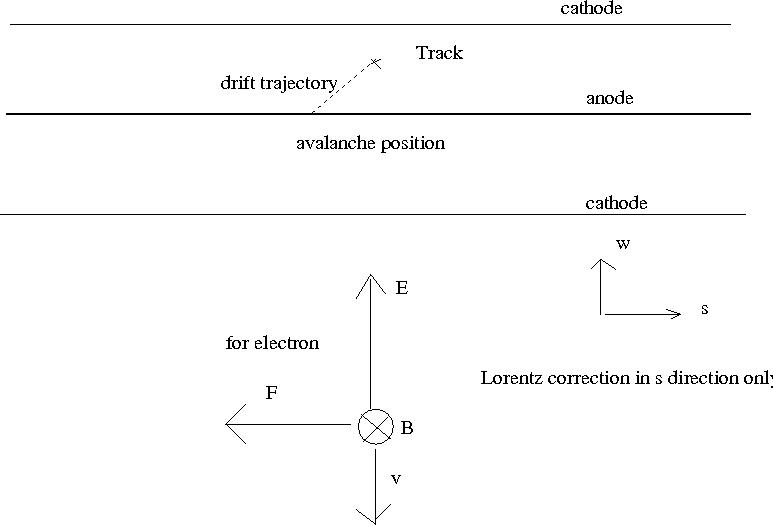
\includegraphics[height=6cm]{FDC_cell.jpg}
$$
\bcent
drift cell with B field normal to wire plane
\ecent
}

\frame{
\frametitle{Runnning Simon's Code}
\bitem
\item run HDGEANT with Simon's configuration
  \bitem
  \item one charged pion(?)
  \item may or may not hit all layers of the FDC
  \eitem
\item run S.'s reconstruction
  \bitem
    \item helical Riemann fit
    \item local L-R ambiguity resolution(?) 
  \eitem
\item make S.'s histograms
\eitem
}

\frame{
\frametitle{Residuals without Lorentz correction}
$$
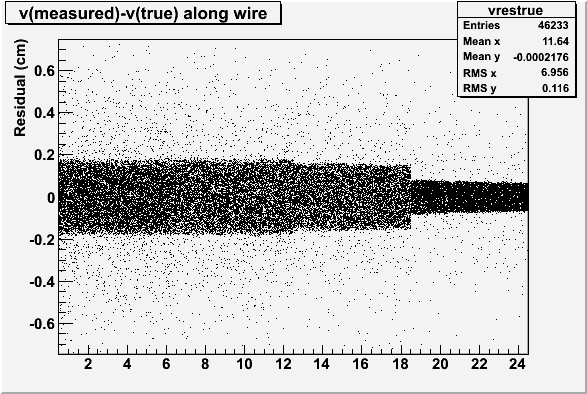
\includegraphics[height=6cm]{vres_simon_binary1.png}
$$
\bcent
residuals vs. FDC layer
\ecent
}

\frame{
\frametitle{Residuals with Lorentz correction}
$$
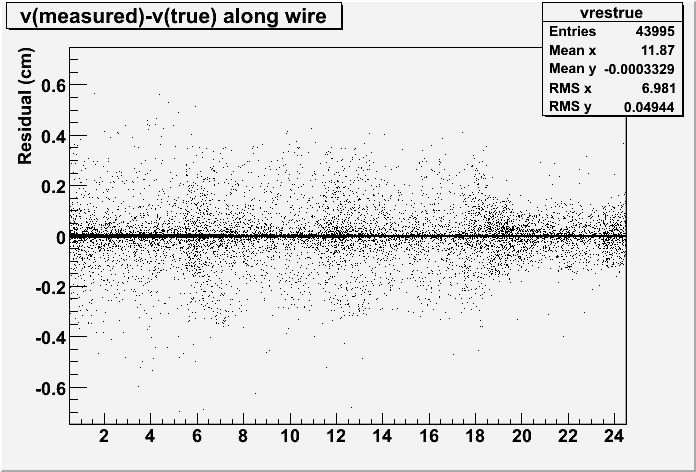
\includegraphics[height=6cm]{vres_good_roentgen.png}
$$
\bcent
residuals vs. FDC layer
\ecent
}

\frame{
\frametitle{Single Event Display}
\bitem
\item FDC hits are rendered as 3-D space points
  \bitem
  \item both cathode planes and anode wire combined into single point (aka psuedopoint)
  \item drift time taken into account
  \item Lorentz correction applied
  \item both depend on L-R choice
  \eitem
\item events with bad residuals easy to find
  \bitem
  \item event 39 is an example
  \eitem
\eitem
}

\frame{
\frametitle{Event 39, with drift times and Lorentz correction}
$$
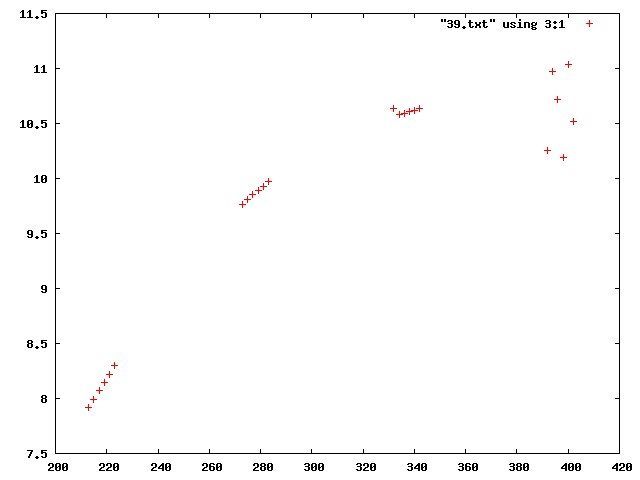
\includegraphics[height=6cm]{39xz.jpg}
$$
\bcent
x vs. z (cm)
\ecent
}

\frame{
\frametitle{Event 39, with drift times and Lorentz correction}
$$
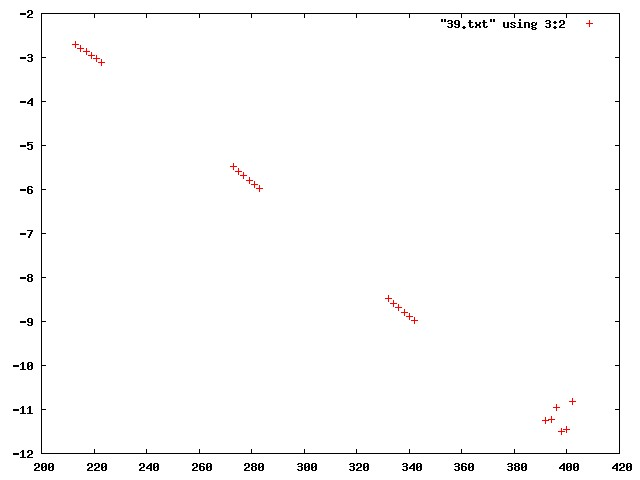
\includegraphics[height=6cm]{39yz.jpg}
$$
\bcent
y vs. z (cm)
\ecent
}

\frame{
\frametitle{Event 39, with drift times and Lorentz correction}
$$
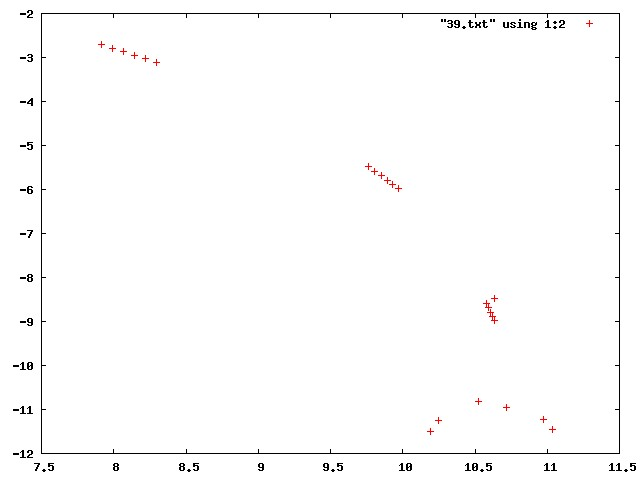
\includegraphics[height=6cm]{39yx.jpg}
$$
\bcent
y vs. x (cm)
\ecent
}

\frame{
\frametitle{alternate hit positions}
\bitem
\item apply drift time correction and Lorentz correction with opposite sign
\item gives an apparent shift from original corrected point
\item also try opposite shift (?!)
\eitem
}

\frame{
\frametitle{Event 39, package 3, close-up}
$$
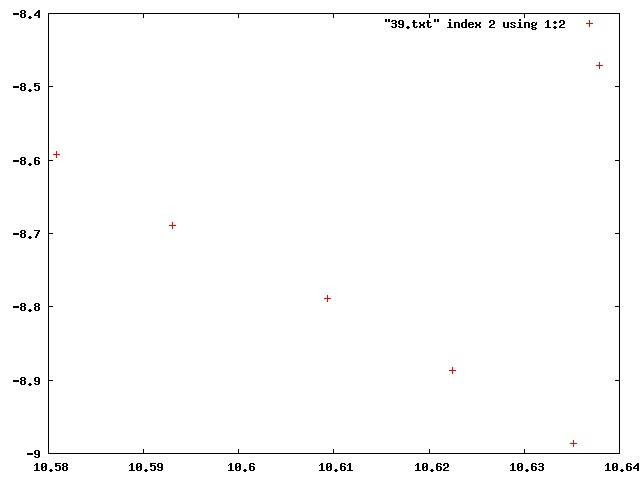
\includegraphics[height=6cm]{39p3_plain.jpg}
$$
\bcent
y vs. x (cm)
\ecent
}

\frame{
\frametitle{Event 39, package 3, alternate choices}
$$
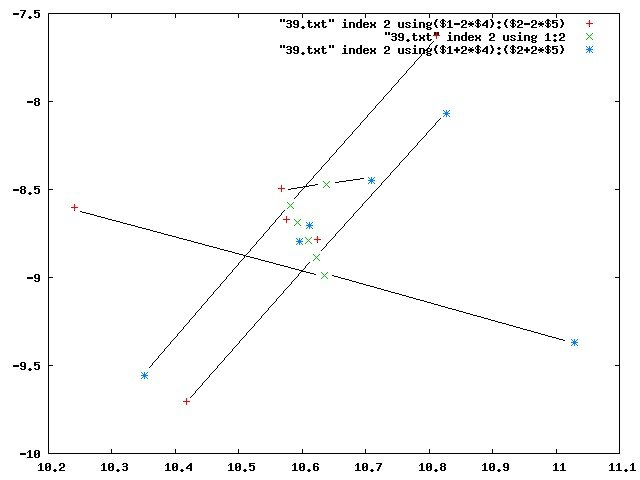
\includegraphics[height=6cm]{39p3_fix.jpg}
$$
\bcent
y vs. x (cm)
\ecent
}

\frame{
\frametitle{Event 39, package 4, close-up}
$$
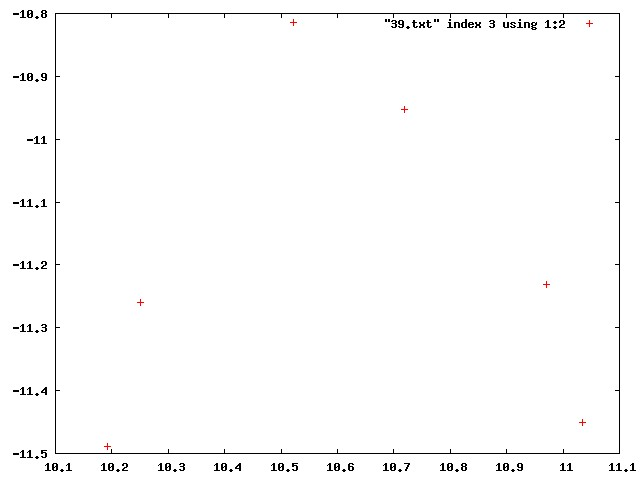
\includegraphics[height=6cm]{39p4_plain.jpg}
$$
\bcent
y vs. x (cm)
\ecent
}

\frame{
\frametitle{Event 39, package 4, alternate choices}
$$
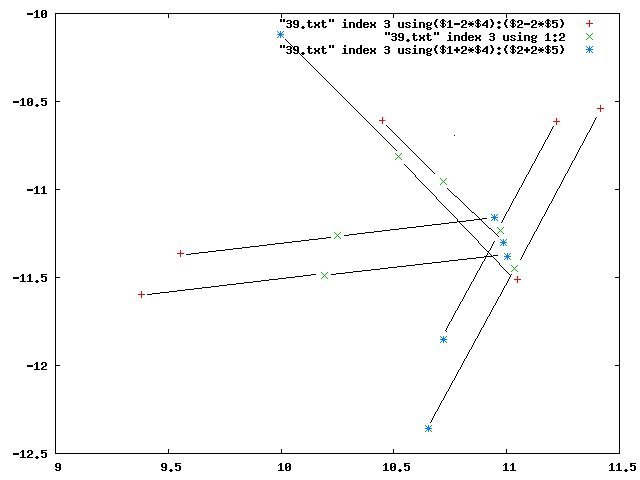
\includegraphics[height=6cm]{39p4_fix.jpg}
$$
\bcent
y vs. x (cm)
\ecent
}

\frame{
\frametitle{Conclusions thus far...}
\bitem
\item wrong choice in resolving L-R ambiguity can lead to large residuals
\item This can be corrected: not intrinsic flaw in chamber
\item The above says nothing about material budget
\item Mystery: alternate alternate choice
  \bitem
  \item Should only be a two-fold ambiguity, not three-way
  \eitem
\item More work needed
  \bitem
  \item tweak Simon's?
  \item different approach?
  \eitem
\eitem
}

\end{document}

%%% end of latex file %%%%
